\chapter{Risultati}
\label{cap:risultati}

In questo capitolo si presenta un'analisi dettagliata dei risultati ottenuti dagli esperimenti descritti in precedenza.

\section{Risultati degli Esperimenti QUIC}
\subsection{Risultati Esperimento 1}
~\\
\indent In questa sezione si analizzano i risultati ottenuti dall'esperimento in cui si è simulato un \emph{server web QUIC} con un comportamento modificato, vedi sezione \ref{esperimento1}.
Il \emph{server} è configurato per operare come se non ricevesse mai conferme dei pacchetti inviati, mantenendo al contempo un \emph{PTO} impostato a 0. 
Di seguito, vengono presentati i risultati emersi accompagnati dai relativi grafici. I dati in versione tabellare sono presenti nell'Appendice.
\\\\
In condizioni standard, la trasmissione ha generato un traffico di circa 5.8 \emph{Mb} con un totale di circa 4100 pacchetti scambiati. 
Questi dati rappresentano il punto di riferimento per valutare l'impatto dei cambiamenti al comportamento del \emph{server}.
\\\\
Come illustrato in Figura \ref{grafico12}, che mostra il confronto del consumo dati tra i vari esperimenti e lo scenario standard, le modifiche hanno prodotto effetti considerevolmente diversi.
Negli scenari di \emph{Retransmission 1 e 2} si è osservato un incremento del traffico dati di più del $100\%$, passando dai 5.8 \emph{Mb} dello scenario standard a circa 13 \emph{Mb} nel primo caso e 15 \emph{Mb} nel secondo. 
Parallelamente, come viene evidenziato in Figura \ref{grafico1}, il numero di pacchetti scambiati è aumentato da 4100 a circa 18000. 
Tuttavia, questi scenari hanno presentato problemi di congestione e latenza che ne hanno compromesso l'applicabilità pratica.
\\\\
Le varianti 4 e 5 hanno mostrato un comportamento differente, principalmente grazie alla modifica che permette l'accettazione di un \emph{ACK} ogni due ricevuti.
La variante 4, che non ignora la richiesta di chiusura della connessione, ha registrato un consumo di 58 \emph{Mb} e circa 65000 pacchetti, senza causare latenza o congestioni. 
La variante 5, che invece blocca le richieste di chiusura della connessione, ha mostrato un consumo di 29 \emph{Mb} e circa 35000 pacchetti, manifestando una latenza minima nel caricamento dei contenuti.

\begin{figure}[!h]
    \centering
    \begin{minipage}{0.48\textwidth}
        \centering
        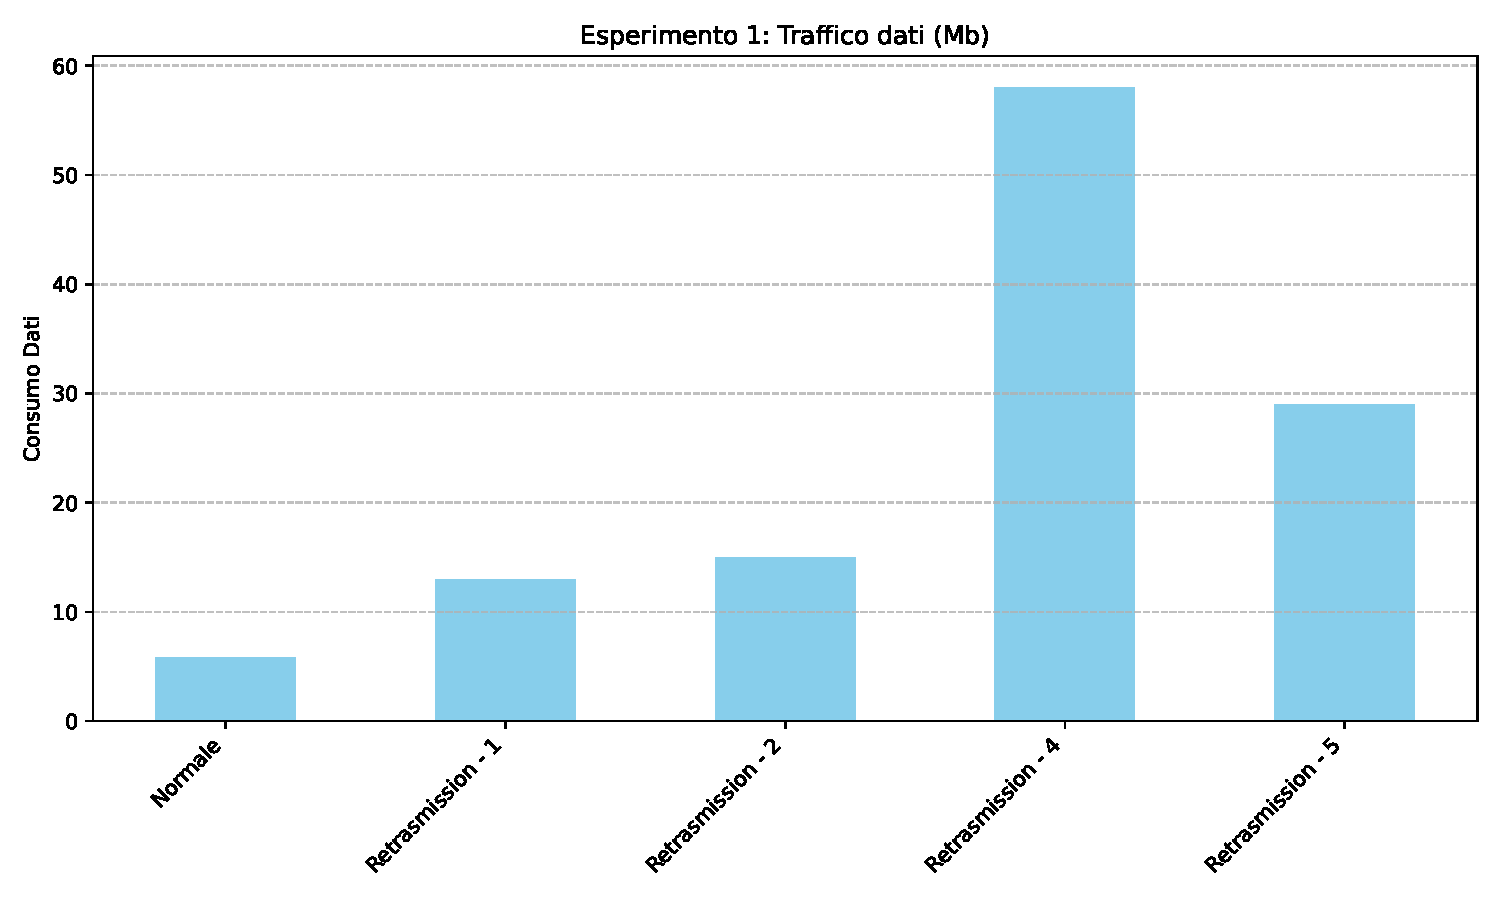
\includegraphics[width=\textwidth]{graphTraffico1.pdf}
        \caption{\emph{Traffico Dati (Mb)}}
        \subcaption*{Consumo totale del traffico dati di ogni esperimento in confronto alla connessione standard.}
        \label{grafico12}
    \end{minipage}
    \hfill
    \begin{minipage}{0.48\textwidth}
        \centering
        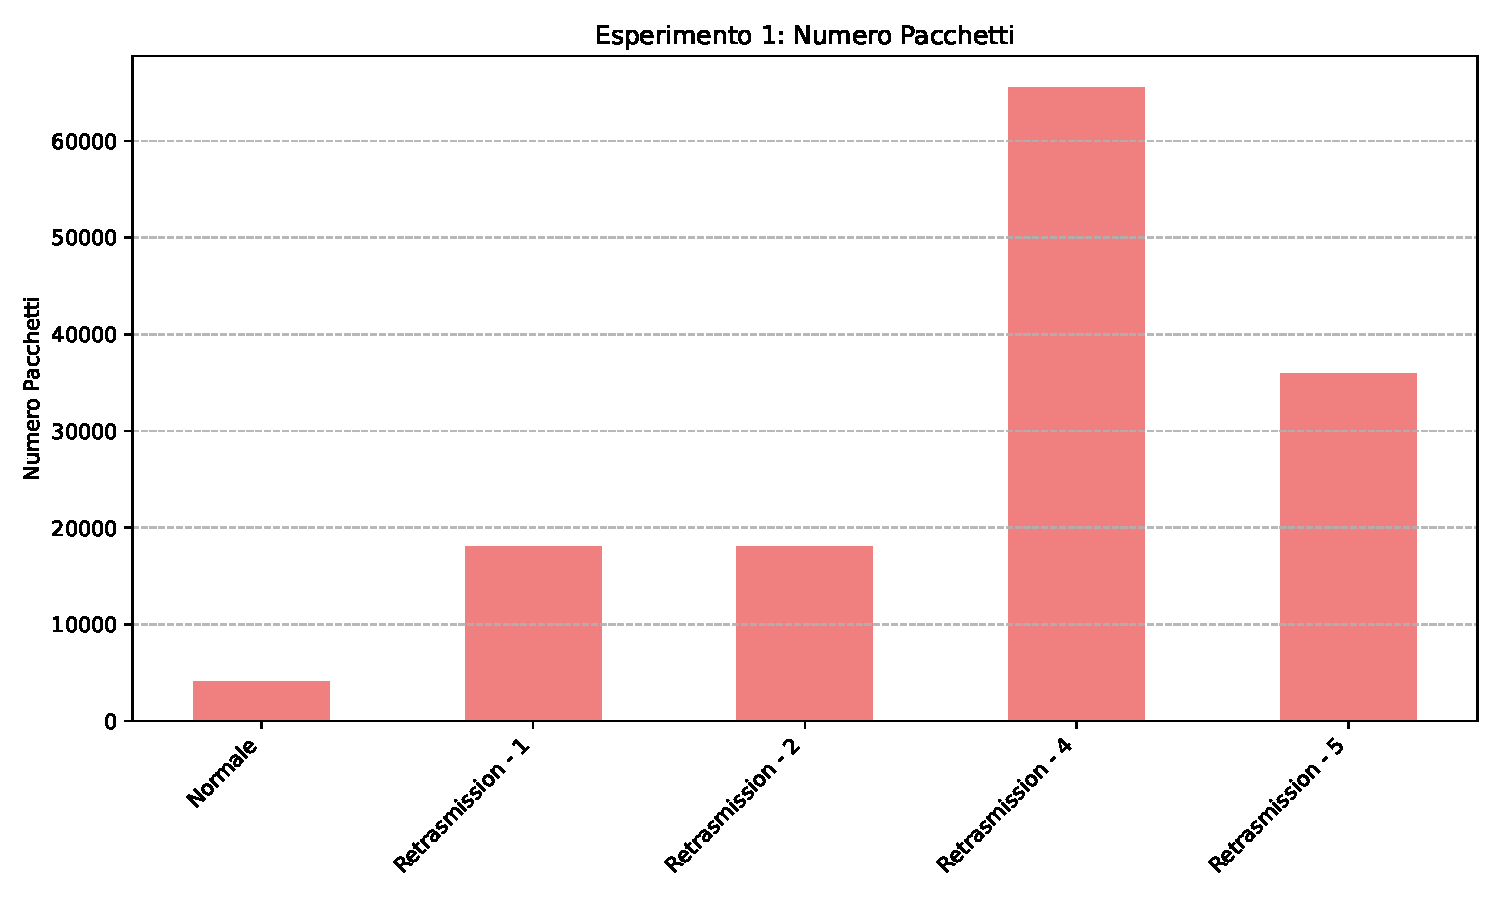
\includegraphics[width=\textwidth]{graphNumPacchetti1.pdf}
        \caption{\emph{Pacchetti Trasmessi}}
        \subcaption*{Numero totale di pacchetti inviati in una connessione per ogni esperimento in confronto alla connessione normale.}
        \label{grafico1}
    \end{minipage}
\end{figure}
\noindent I risultati evidenziano come la gestione degli \emph{ACK} unita ad un \emph{PTO} costante a 0 influenzi significativamente sia il consumo di dati che il numero di pacchetti scambiati.
La variante 4 in particolare, incrementa il traffico dati di dieci volte, passando da 5.8 Mb a 58 Mb, e il numero di pacchetti da 4100 a 65500, senza però introdurre latenza o congestione. 
Tutto questo implica che, pur mantenendo una connessione all'apparenza normale, le modifiche comportino un potenziale aumento significativo del traffico contabilizzato per l'utente.
\subsection{Risultati Esperimento 2}
~\\
\indent In questa sezione si analizzano i risultati ottenuti dall'esperimento in cui si è simulato un \emph{server web QUIC} che inietta pacchetti aggiuntivi non richiesti in background, vedi sezione \ref{esperimento2}.
Il \emph{server} è stato configurato per mantenere una connessione \emph{QUIC} standard con il \emph{client}, mentre contemporaneamente invia pacchetti aggiuntivi non correlati alla comunicazione principale.
\\\\
I risultati dell'esperimento illustrati nelle Figure \ref{grafico22} e \ref{grafico2}, mostrano gli effetti dell'iniezione di pacchetti sul consumo di dati e sul volume del traffico in termini di pacchetti scambiati.
Come punto di riferimento si ha che la connessione \emph{QUIC} standard genera un traffico di circa 5.8 \emph{Mb} con 4100 pacchetti scambiati.
\\\\
L'introduzione dell'iniezione di pacchetti ha portato a un aumento prevedibile sia nel volume di traffico che nel numero di pacchetti.
Nel primo scenario \emph{(Inject - 1)}, con 6 \emph{worker} che inviano 1000 pacchetti al secondo, si è ottenuto un aumento significativo del traffico raggiungendo circa 272 \emph{Mb} e quasi 190'000 pacchetti scambiati in 30 secondi. 
Aumentando la frequenza di invio a 2000 pacchetti al secondo \emph{(Inject - 2)} e mantendo sempre a 6 i \emph{workers}, il traffico è quasi raddoppiato, arrivando a circa 566 \emph{Mb} con 396'000 pacchetti.
\\\\
Nel terzo scenario \emph{(Inject - 3)}, aumentando i \emph{worker} a 8 ma mantenendo i pacchetti al secondo a 1000, si è ottenuto un aumento del consumo dati di circa 407 \emph{Mb} e 535'000 pacchetti. 
Infine nella quarta variante \emph{(Inject - 4)}, combinando 8 \emph{worker} e una frequenza di invio di 2000 pacchetti al secondo, si è ottenuto il picco di circa 753 \emph{Mb}, con 543'000 pacchetti.
\begin{figure}[!h]
    \centering
    \begin{minipage}{0.48\textwidth}
        \centering
        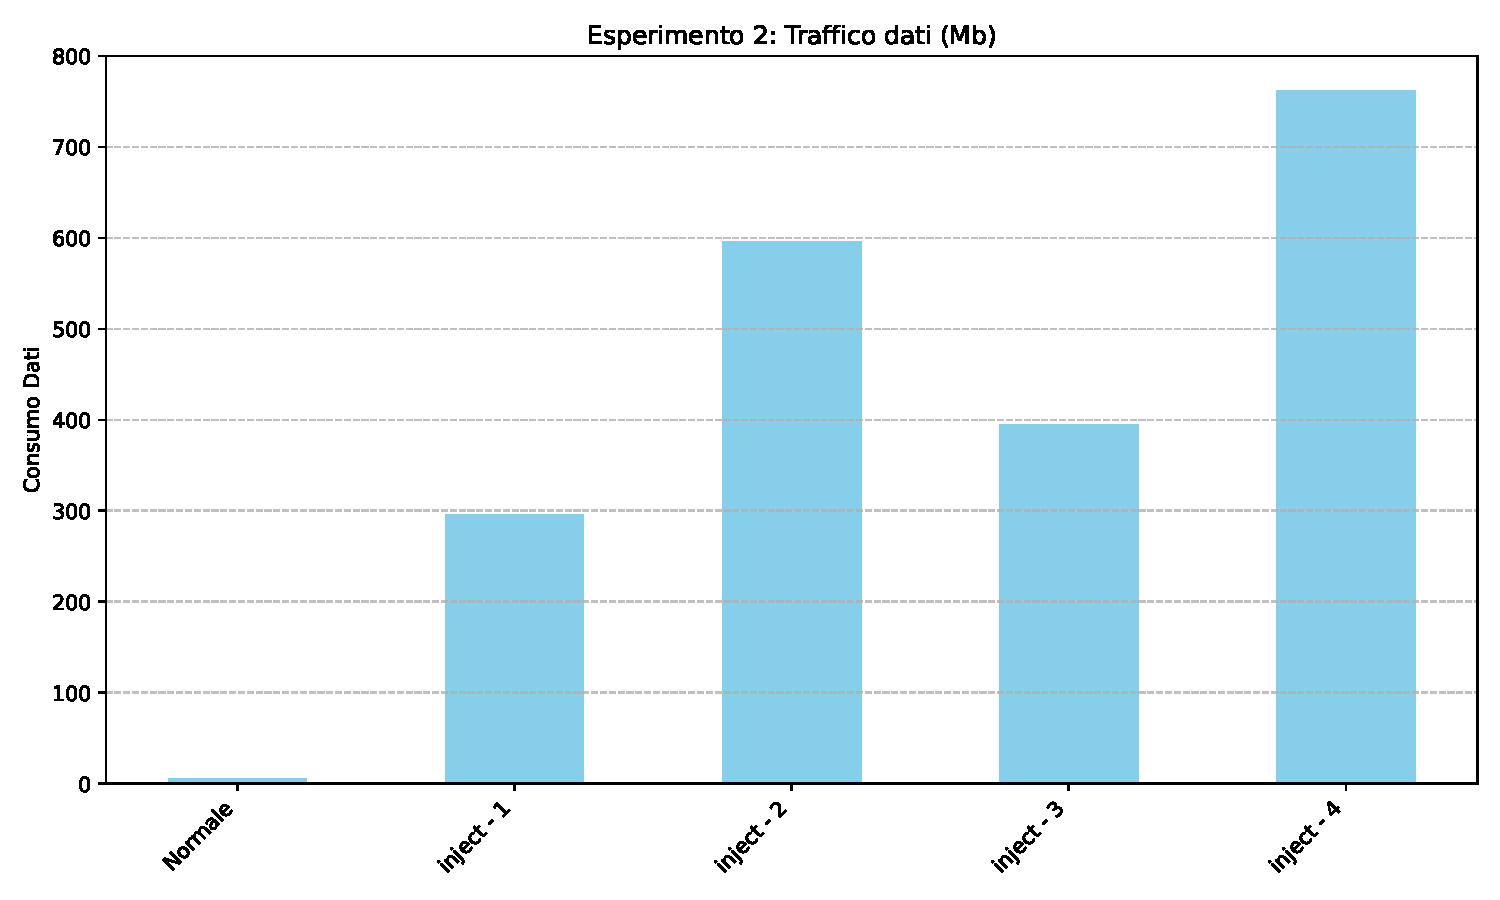
\includegraphics[width=\textwidth]{graphTraffico2.pdf}
        \caption{\emph{Traffico Dati (Mb)}}
        \subcaption*{Consumo totale del traffico dati di ogni esperimento in confronto alla connessione standard in 30 secondi.}
        \label{grafico22}
    \end{minipage}
    \hfill
    \begin{minipage}{0.48\textwidth}
        \centering
        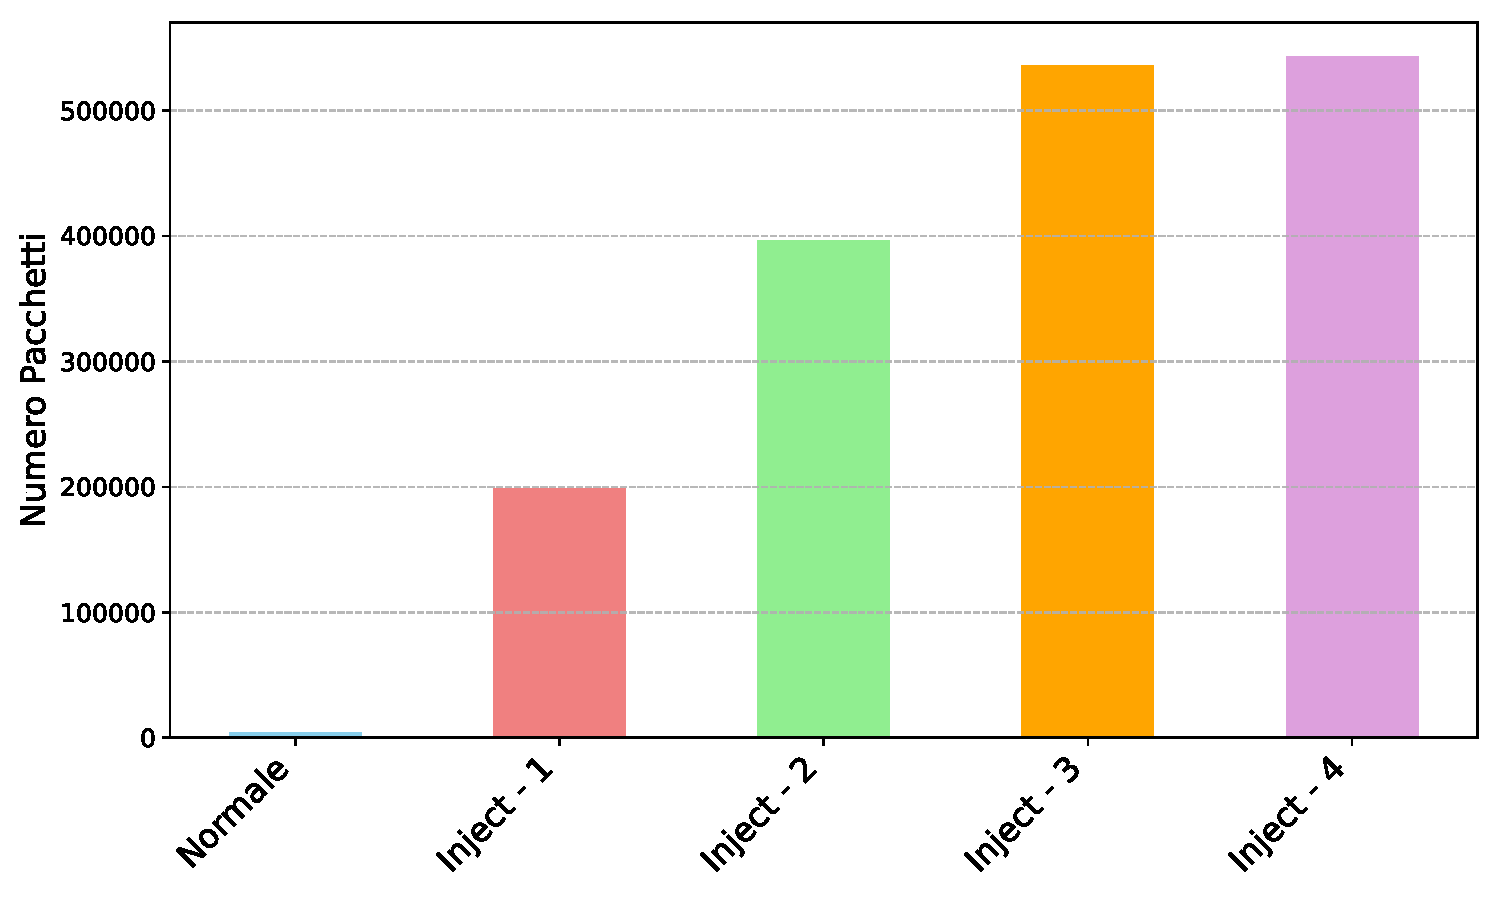
\includegraphics[width=\textwidth]{graphNumPacchetti2.pdf}
        \caption{\emph{Pacchetti Trasmessi}}
        \subcaption*{Numero totale di pacchetti inviati in una connessione per ogni esperimento in confronto alla connessione normale in 30 secondi.}
        \label{grafico2}
    \end{minipage}
\end{figure}
\\
\noindent Da sottolineare che l'ambiente di test è locale e via cavo. È proprio per questa ragione che non si sono sperimentati né congestione né latenza durante gli esperimenti. 
In uno scenario di rete reale, con connessioni \emph{wireless} o su lunghe distanze, ci si aspetterebbe la presenza di latenza o congestione, soprattutto considerando gli elevati volumi di traffico generati. 
\begin{figure}[!h]
    \centering
        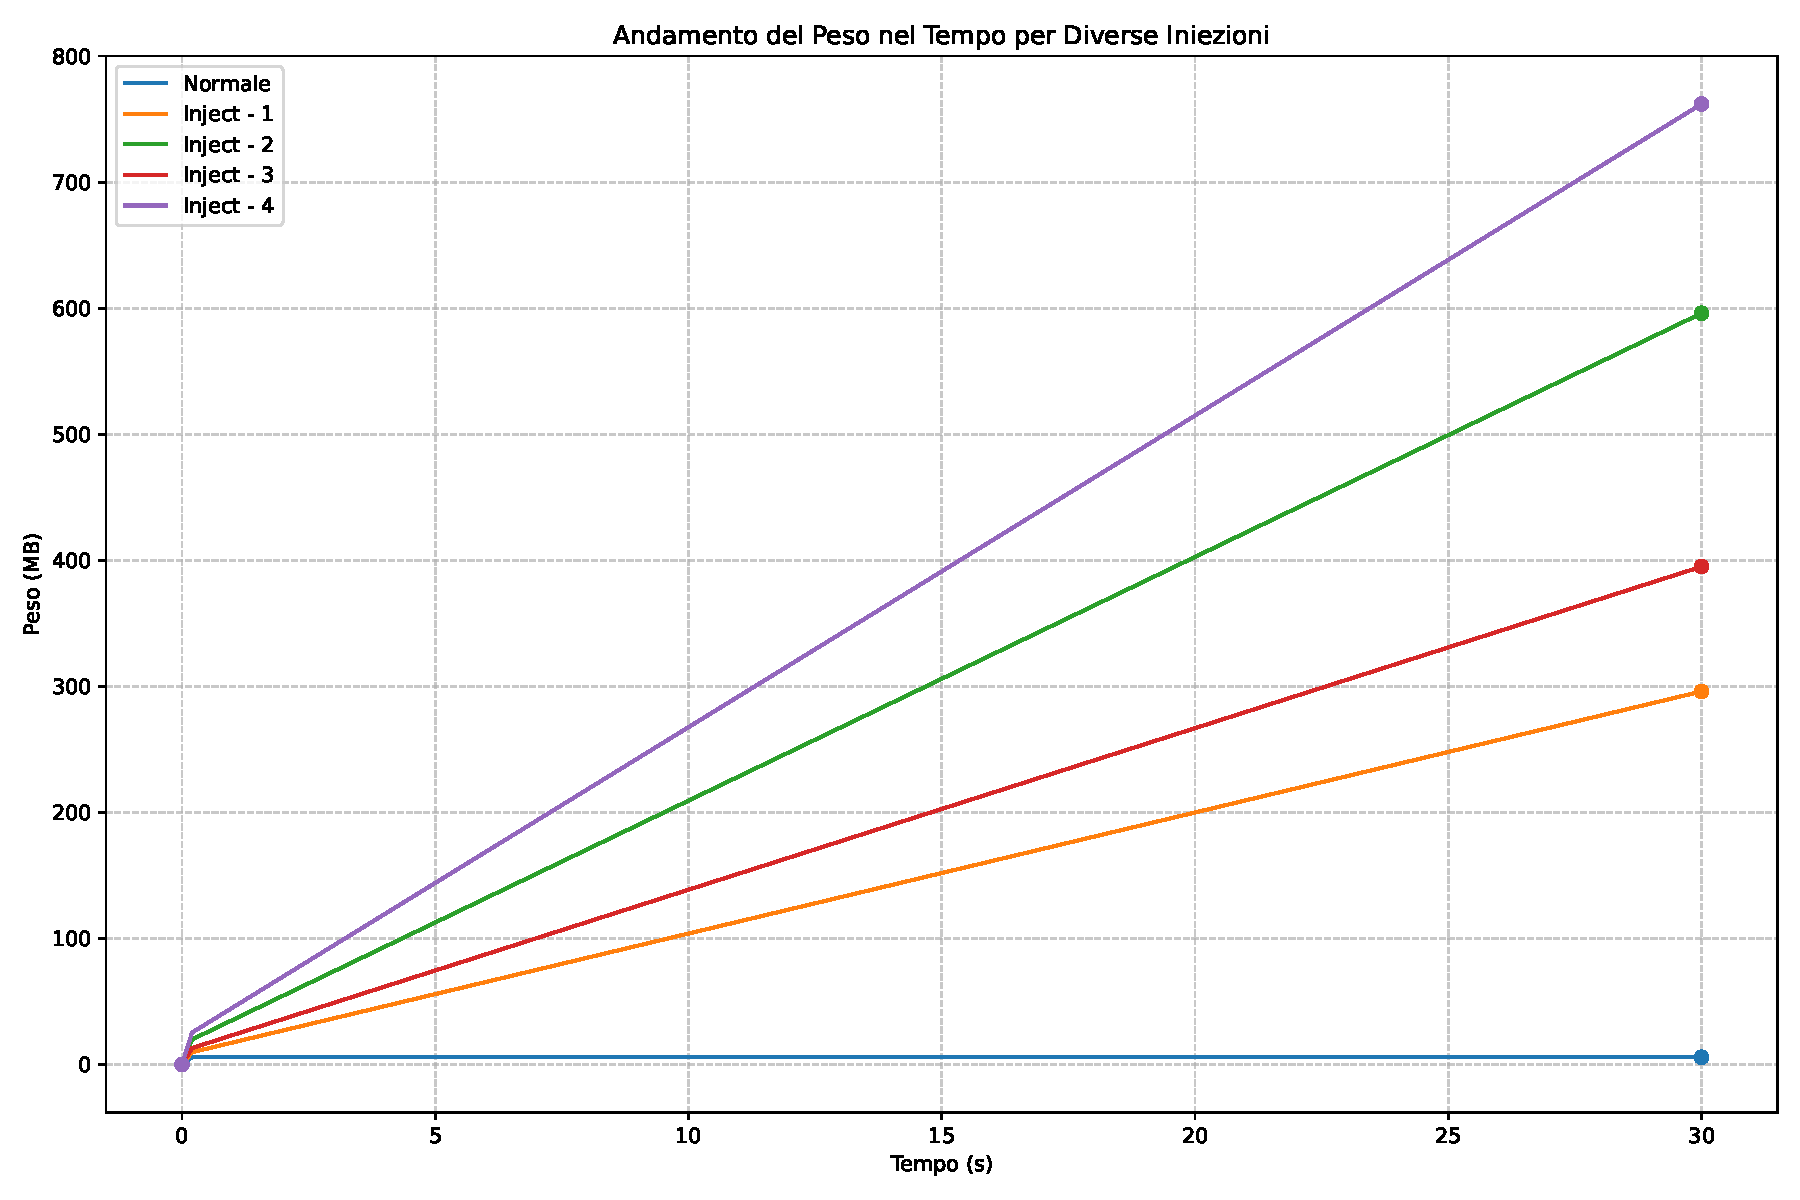
\includegraphics[width=\textwidth]{graphTrafficoTempo.pdf}
        \caption{\emph{Andamento del Consumo Dati nel Tempo}}
        \subcaption*{Andamento del consumo dati di ogni esperimento in confronto alla connessione normale in 30 secondi.}
        \label{grafico23}
\end{figure}
\\\\
\noindent A differenza dei risultati dell'esperimento 1, in questo caso il volume di traffico risulta costante.
Mentre nel primo scenario il volume era influenzato dalla variabile del peso della connessione principale, in questo esperimento tale fattore diventa irrilevante,
poichè i pacchetti vengono inviati con una frequenza costante, indipendentemente dagli altri parametri.
\\\\
Ciò che assume particolare rilevanza è la durata in cui la connessione rimane attiva, poiché essa determina la quantità totale di pacchetti che possono essere inviati.
Nell'esperimento che si è condotto, la connessione è stata simulata per una durata di 30 secondi. 
La Figura \ref{grafico23} illustra l'andamento dei singoli esperimenti a paragone con quello della connessione standard nel medesimo intervallo di tempo.

\subsection{Risultati Esperimento 3}
~\\
\indent In questa sezione si analizzano i risultati ottenuti dall’esperimento in cui si è simulato
uno scenario di attacco in cui un attaccante esterno cerca di manipolare il traffico di una connessione \emph{QUIC} tra un \emph{client} e \emph{server}, vedi sezione \ref{esperimento3}.
L'attacco si concentra sull'oscuramento selettivo di pacchetti con lo scopo di causare ritrasmissioni e aumentare il traffico.
\\\\
I risultati dell'esperimento, riportati nelle Figure \ref{grafico3} e \ref{grafico32}, mostrano l'efficacia del pattern di selezione applicato per determinare quali pacchetti oscurare. 
Nel primo scenario \emph{(Spurious Retransmission - 1)}, l'attacco è stato eseguito bloccando tutti i pacchetti nella connessione inferiori a 85 \emph{byte}, avendo come effetto un totale blocco della risorsa.
Ciò ha impedito qualsiasi accesso al \emph{server web}, nonostante questo sia un risultato significativo per un possibile attaccante non è rilevante per lo scopo di questo studio che invece cerca di aumentare il traffico.
\\\\
Nel secondo scenario \emph{(Spurious Retransmission - 2)} si è oscurato un pacchetto ogni due con dimensioni inferiori a 85 \emph{byte}. Ciò ha portato a un incremento di circa il 10\% nel numero di pacchetti, senza tuttavia creare alcuna latenza o congestione.
Aumentando la frequenza di oscuramento a due ogni tre \emph{(Spurious Retransmission - 3)} si è causato un aumento del numero di pacchetti del 30\% rispetto alla connessione normale, con un consumo totale di 6.6 \emph{Mb} e 5377 pacchetti scambiati.
\begin{figure}[ht]
    \centering
    \begin{minipage}{0.48\textwidth}
        \centering
        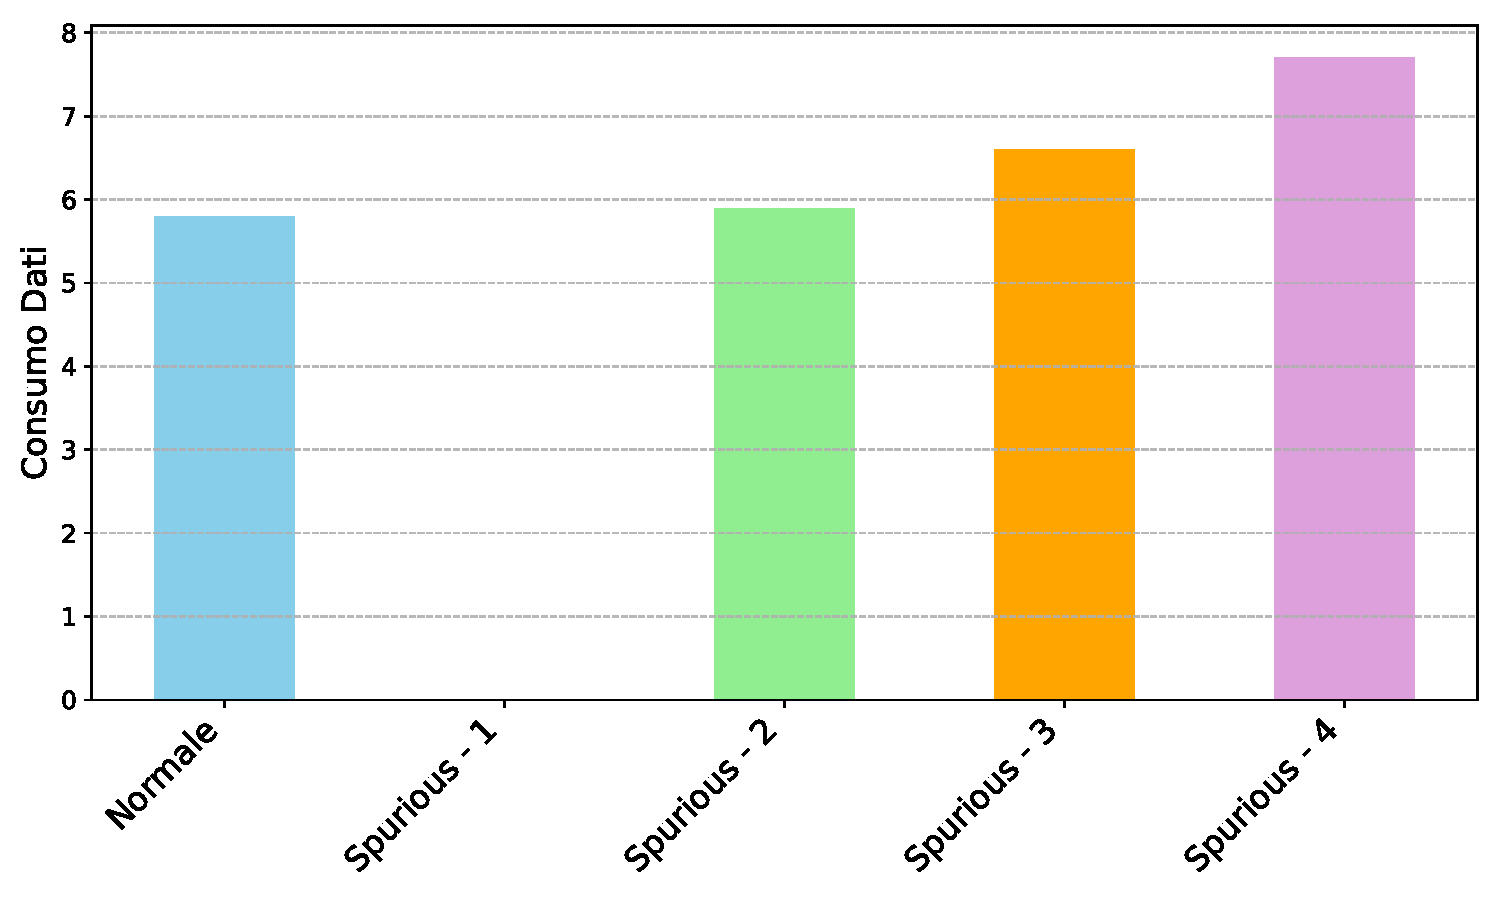
\includegraphics[width=\textwidth]{graphTraffico3.pdf}
        \caption{\emph{Traffico Dati (Mb)}}
        \subcaption*{Consumo totale del traffico dati di ogni esperimento in confronto alla connessione normale.}
        \label{grafico3}
    \end{minipage}
    \hfill
    \begin{minipage}{0.48\textwidth}
        \centering 
        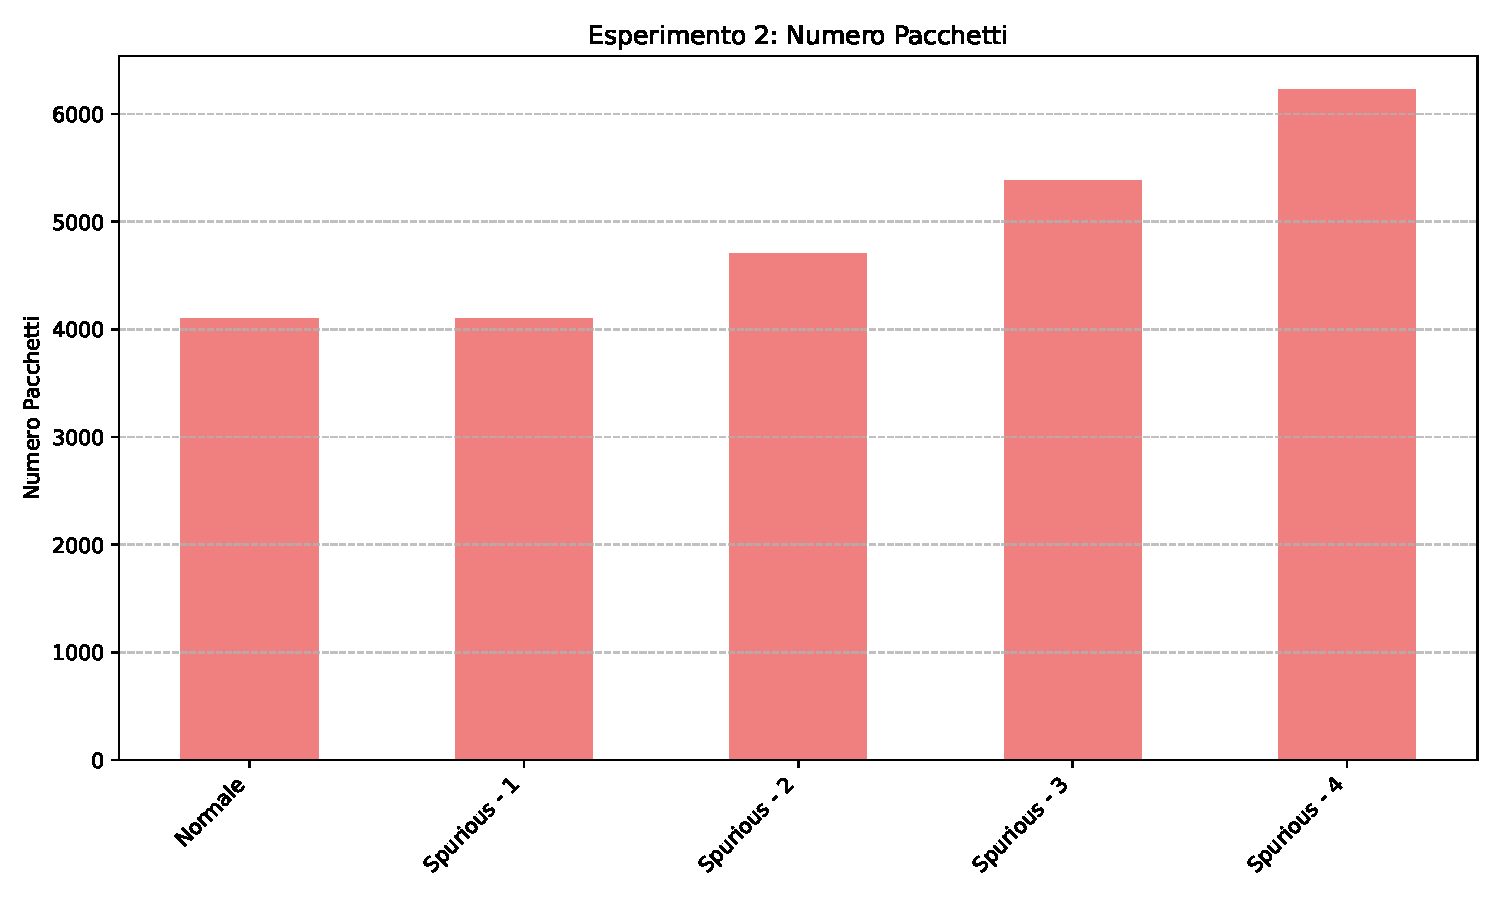
\includegraphics[width=\textwidth]{graphNumPacchetti3.pdf}
        \caption{\emph{Pacchetti Trasmessi}}
        \subcaption*{Numero totale di pacchetti inviati in una connessione per ogni esperimento in confronto alla connessione normale.}
        \label{grafico32}
    \end{minipage}
\end{figure}
Nel quarto e ultimo scenario \emph{(Spurious Retransmission - 4)} sono stati oscurati quattro pacchetti su cinque, sempre selezionando quelli inferiori a 85 \emph{byte}.
Questo ha portato un aumento del numero di pacchetti quasi del 50\%, con un totale di poco meno di 8 \emph{Mb} e 6200 pacchetti scambiati.